\documentclass{article}%
\usepackage[T1]{fontenc}%
\usepackage[utf8]{inputenc}%
\usepackage{lmodern}%
\usepackage{textcomp}%
\usepackage{lastpage}%
\usepackage[head=40pt,margin=0.5in,bottom=0.6in]{geometry}%
\usepackage{graphicx}%
%
\title{\textbf{Jubilados de Cantv exigen mejores condiciones por sus años de servicio}}%
\author{EL NACIONAL WEB}%
\date{25/09/2018}%
%
\begin{document}%
\normalsize%
\maketitle%
\textbf{URL: }%
http://www.el{-}nacional.com/noticias/politica/jubilados{-}cantv{-}exigen{-}mejores{-}condiciones{-}por{-}sus{-}anos{-}servicio\_253142\newline%
%
\textbf{Periodico: }%
EN, %
ID: %
253142, %
Seccion: %
Política\newline%
%
\textbf{Palabras Claves: }%
Política, Delcy Rodríguez, Estados Unidos, Cilia Flores, Jorge Rodríguez, Vladimir Padrino López\newline%
%
\textbf{Derecho: }%
2.6%
, Otros Derechos: %
NO\_TIENE%
, Sub Derechos: %
2.6.1%
\newline%
%
\textbf{EP: }%
SI\newline%
\newline%
%
\textbf{\textit{Los trabajadores retirados de la empresa trancaron la avenida Libertador para exigir mejores condiciones en sus pensiones}}%
\newline%
\newline%
%
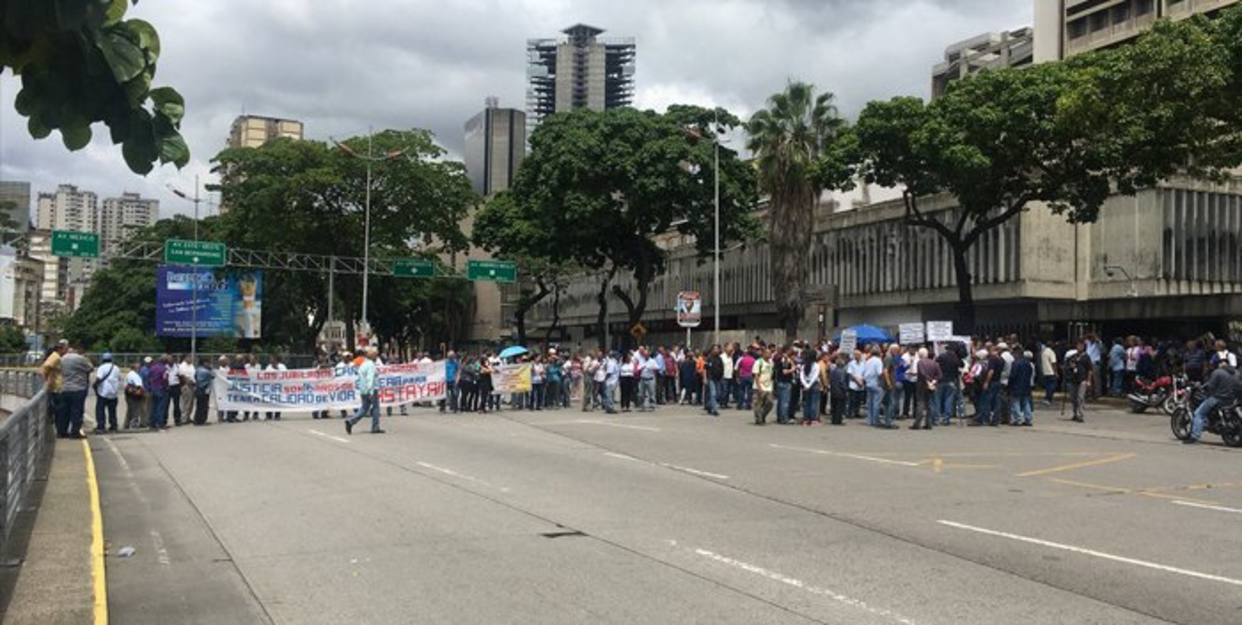
\includegraphics[width=300px]{102.jpg}%
\newline%
%
Jubilados de Cantv protestan este martes, en la avenida Libertador de~Caracas, para exigir mejores condiciones por sus años de servicio en~la empresa.%
\newline%
%
Los manifestantes trancaron el paso de vehículos en la avenida y piden que se les otorgue un servicio médico para sobrevivientes, se homologuen sus pensiones y se les otorgue el mismo bono de alimentación que reciben los trabajadores activos.%
\newline%
%
Por medio de carteles, denuncian que luego de 16 años de trabajo en Cantv no tienen una calidad de vida digna por las precarias pensiones que reciben.%
\newline%
%
\end{document}